%!TEX root = ../report.tex

% 
% Related work
% 

\section{Related Work}

% Example citation:
In this section we will present a set of literature references on the subjects related to this thesis. We will present the most important frameworks on Information Systems Management and Governance. This process has the objective to come up with a choice of a frameworks or a set of them to implement our processes for project and maintenance management\par
In terms of logical application architectures, we will provide an analysis of the main features of a set of Project Management and Information Technologies Service Management solutions available in the market. Our objective is to conduct an comparative analysis relating all the solutions and choose the ones that best fit our purposes for use on an logical application architecture.  

\subsection{Frameworks for Information Technologies Governance and Management}

In this section we will present the three frameworks we consider the most relevant for this thesis: COBIT 5, ITIL V3 and PMBOK. This three frameworks provide, from different perspectives, guides and principles for IT Governance and Management, providing processes for achieving a successful implementation of this principles in an organization.\par


\subsubsection{IT Governance and IT Management}

One important concept to define is the difference between IT Governance and IT management. They are many times confused and some authors already tried to explain the difference between the two concepts.\par
Considering the definition given by Van Grembergen \textit{et al.}, ``''IT Management is focused on the internal effective supply of IT services and products and the management of present IT operations. IT Governance in turn is much broader, and concentrates on performing and transforming IT to meet present and future demands of the business (internal focus) and the business´ customers (external focus).``''.\par
 Considering the COBIT 5 view for this question, it makes a clear distinction between governance and management, in the way these two disciplines encompass different types of activities, require different organizational structures and serve different purposes.\par
 Governance ensures that stakeholder needs, conditions and options are evaluated to determine balanced, agreed-on enterprise objectives to be achieved; setting direction through prioritisation and decision making; and monitoring performance and compliance against agreed-on direction and objectives.Management plans, builds, runs and monitors activities in alignment with the direction set by the governance body to achieve the enterprise objectives.\par

\begin{figure}
\centering
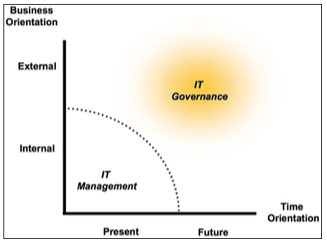
\includegraphics[width=0.6\textwidth]{img/ITGovernanceAndManagement.png}
\caption{IT Governance and IT Management}
\end{figure}


 Considering both definitions and the figure 1, we can conclude that IT Governance has a bigger dimension that IT Management, but are disciplines that need to be related and complementary to achieve success inside an organization.

\subsubsection{COBIT 5}

Control Objectives for Information and Related Technology (COBIT) is a framework created by the Information Systems Audit and Control Association (ISACA) for IT Management and IT Governance.\par
COBIT 5 provides a comprehensive framework that assists enterprises in achieving their objectives for the governance and management of enterprise IT. Simply stated, it helps enterprises create optimal value from IT by maintaining a balance between realizing benefits and optimizing risk levels and resource use \cite{2012cobit}. 
The framework is built on five basic principles:

\begin{itemize}
  \item \textbf{Meeting the Stakeholders Needs} 
  \item \textbf{Covering the Enterprise End-to-end} 
  \item \textbf{Applying a Single, Integrated Framework} 
  \item \textbf{Enabling a Holistic Approach} 
  \item \textbf{Separating Governance from Management}
\end{itemize}


It also defines seven enablers, explained by COBIT as factors that, individually and collectively, influence whether governance and management over enterprise will work or not. This enablers can be categorized as:

\begin{itemize}
  \item \textbf{Principles, Policies and frameworks} 
  \item \textbf{Processes} 
  \item \textbf{Organizational structures} 
  \item \textbf{Culture, ethics and behavior} 
  \item \textbf{Information}
  \item \textbf{Services, infrastructure and applications} 
  \item \textbf{People, skills and competencies}
\end{itemize}

\begin{figure}
\centering
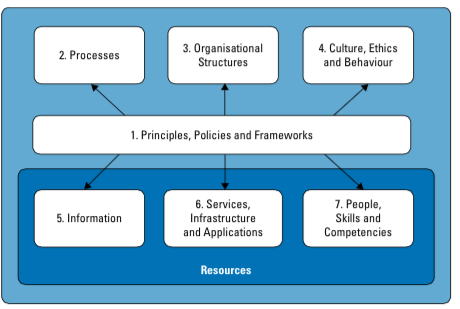
\includegraphics[width=0.7\textwidth]{img/Enablers.png}
\caption{COBIT 5 enablers}
\end{figure}

Image 2 presents the COBIT 5 enablers previous defined and how they relate among themselves int terms of its importance for organization. Each enabler has stakeholders, a set of goals, a life cycle and for each can be defined good practices.\par

\begin{figure}
\centering
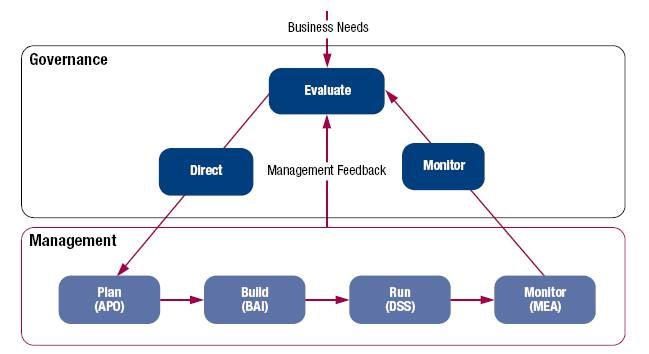
\includegraphics[width=0.9\textwidth]{img/COBITProcesses.jpg}
\caption{COBIT 5 domains}
\end{figure}

Considering figure 3, COBIT 5 process reference model considers two big domains of processes: Governance and Management. The governance domain contains five processes in the domain evaluate, direct and monitor(EDM). The management domain has four internal domains of processes:Align, Plan and Organise(APO), Build, Acquire and Implement(BAI), Deliver, Service and Support (DSS) and Monitor, Evaluate and Assess(MEA).\par
All processes for management and governance are presented in the appendix and all the implementation details are presented in COBIT 5: Enabling Processes.[REFERENCE HERE]\par
COBIT 5 includes a process capability model based on ISO/IEC 15504 Sotware Engineering - Process Assessment standard. [REFERENCE HERE] This models allow to measure the current level of maturity of enterprise processes, presenting the gap between the current level and the desired one the enterprise wants to achieve. This new capability model is an improvement of the previous on COBIT 4.1, being more simplified and compliant with a generally accepted process assessment standard.
Relating to other frameworks and standards, COBIT tries to establish a framework that is compliant with the most widely accepted standards in IT Governance and Management. In figure 4 we can see the standards COBIT 5 relates by processes domain, with special attention to ITIL V3, ISO/IEC 20000, PMBOK and CMMI, that are closely related to this thesis problem.

\cite{*}






